\documentclass[french]{article}

% Page
    \usepackage[a4paper,%
            left=1in,right=1in,top=1in,bottom=1in]{geometry}
    \usepackage{lscape}

% Abstract
    \usepackage{abstract} % Allows abstract customization
    % Set the "Abstract" text to bold
    \renewcommand{\abstractnamefont}{\normalfont\bfseries}
    % Set the abstract itself to small italic text
    \renewcommand{\abstracttextfont}{\normalfont\small\itshape} 

% Title
    \usepackage{titlesec} % Allows customization of titles
    
% Endnotes
	% Uncomment this line if using endnotes "\endnote{}"
	% \usepackage{endnotes}
    
% Headers from page 2 on
    \usepackage{fancyhdr}
    \pagestyle{fancy}
    \fancyhf{}
    \usepackage{lastpage}

% MACROS
    % Define keywords macro command
    \providecommand{\keywords}[1]{\textbf{\textit{Keywords---}} #1}


% MATH SUPPORT
    % The amssymb package provides various useful mathematical symbols
    \usepackage{amssymb}
    % The amsthm package provides extended theorem environments
    \usepackage{amsthm}
    % The newtxmath package provides additional math symbol support
    	% in Times New Roman symbols, etc.
    \usepackage{newtxmath}

% FONTS
    \usepackage{microtype} % Slightly tweak font spacing for aesthetics
    \usepackage[utf8]{inputenc}
    \usepackage{newtxtext} % Makes default font Adobe Times New Roman
    \usepackage[T1]{fontenc}
    \usepackage{rotating}
    \usepackage{babel}
  
% LINES
	% Spacing
	\usepackage{setspace} % See \doublespacing command at the top of content.tex
    % Numbering
    \usepackage{lineno,xcolor} 	% See \linenumbers at the top of content.tex

% COMMENTS
	\usepackage[colorinlistoftodos]{todonotes} % allows margin comments
    % See examples in content.tex, and here for manual: 
    % http://www.ctan.org/pkg/todonotes
	\usepackage{soul} % allows for highlighting

% APPENDIX
    \usepackage[toc,page,title,titletoc,header]{appendix} % pour les annexes
    \renewcommand{\appendixtocname}{Appendices} % indique le nom de la table des annexes dans la toc
    \renewcommand{\appendixpagename}{Appendices} % Nom du titre de la page des annexes

% CODE
    \usepackage{tcolorbox}
    \usepackage{xcolor}
    \newcommand{\reducedstrut}{\vrule width 0pt height .9\ht\strutbox depth .9\dp\strutbox\relax}
    \usepackage{minted}

% SEQUENCES
    \usepackage{texshade}
    \usepackage{booktabs, colortbl}

% GRAPHICS
    \usepackage{svg}
    \usepackage{graphicx} % More advanced figure inclusion
    \usepackage{float} % For specifying table/figure locations, i.e. [ht!]
    
    % The printlen command allows the user to print the exact text width or height.
    % This is useful, when trying to create graphics (outside of LaTeX, of course)
    % with the optimal dimensions. See here for usage: http://www.ctan.org/pkg/printlen
    \usepackage{printlen}
    \usepackage{tikz}
    \usepackage{caption}

% TABLES
    \usepackage{pgfplotstable}
    \pgfplotstableset{
begin table=\begin{longtable},
end table=\end{longtable},
}
    \pgfplotsset{compat=1.17}
    \usepackage{longtable} % For long tables that span multiple pages
    \newcommand{\sym}[1]{\rlap{#1}}% For symbols like *** in tables
    \usepackage{tabularx} % Allows advanced table features
    \newcolumntype{M}{>{\centering\arraybackslash}m{4.4em}}
    \newcolumntype{L}[1]{>{\raggedright\arraybackslash}p{#1}}
    \newcolumntype{C}[1]{>{\centering\arraybackslash}p{#1}}
    \newcolumntype{R}[1]{>{\raggedleft\arraybackslash}p{#1}}
    \usepackage{relsize} % Allows precise adjustment of font size,
    	%useful for fitting tables to page width
    \usepackage{multirow}
    \usepackage{booktabs}
    

% REFERENCES
    \usepackage{cite}
	\usepackage{hyperref} % For hyperlinks in the PDF
	\hypersetup{
	colorlinks=true,
	linkcolor=black,
	citecolor=black,
    urlcolor=blue,
    }
	\usepackage{chicago}

    
 % See preamble.tex to edit the overall layout

\title{Implémentation d'un l'algorithme de Monte Carlo pour le repliement de protéines HP}
\author{Baptiste Rousseau\\ M2-BI Université de Paris Cité}
\date{14 septembre 2022}

\rfoot{Page \thepage \hspace{1pt} of \pageref{sec:end}}

\begin{document}
\maketitle 

\onehalfspacing

\section{Introduction}

Les méthodes de repliement de protéines à partir de leur séquence s'appuient sur la minimisation d'une fonction d'énergie. Les protéines sont des molécules complexes et leur repliement l'est encore plus, c'est pourquoi nous supposons que des perturbations thermiques appliquée à une protéine l'amèneront vers un minimum local d'énergie. Les processus de repliement des protéines in vivo sont guidés, c'est pourquoi nous pouvons imaginer un paysage énergétique en entonnoir contenant un minimum global significatif. Beaucoup de facteurs agissent sur ce paysage énergétique mais nous n'en considérerons ici qu'un. Le modèle HP permet de réduire la complexité des protéines en considérant uniquement le cas de résidus hydrophobiques ou polaires. Ainsi l'objectif sera d'augmenter les interactions entre résidus hydrophobiques.

Afin de minimiser l'énergie l'approche la plus courante est l'utilisation d'un algorithme de Monte Carlo. Cet algorithme suit une descente de gradient mais peut, selon une probabilité, aller à contre-sens. Cela permet ainsi d'échapper aux minima locaux afin d'augmenter les chances du trouver le minimum global. 

\section{Matériels and Méthodes}

Le modèle de séquence sur lequel nous nous appuierons est un modèle dit "Hydrophobe-Polaire" où les acides aminés sont classifiés en deux catégories, "hydrophobes" et "polaire". La séquence HP d'une protéine n'est alors constituée que d'un enchaînement de résidus H et P.

Nous utiliserons le classement ci-suit:
\begin{itemize}
    \item hydrophobes : A I L M F V P G W C
    \item polaires : R N D E Q H K S T Y
\end{itemize}

Ces résidus seront placés sur une grille réduisant ainsi les coordonnées possibles. En plus de cela nous ne considérerons que le cas d'une grille en 2 dimensions. Chaque résidu peut avoir quatre voisins au maximum sur cette grille. L'énergie de conformation associée à cette grille correspond au nombre de contacts directs entre résidus hydrophobes étant voisins topologique, c'est à dire entre résidus voisins n'étant pas consécutifs dans la séquence. Chaque contact aura une contribution négative de -1 à l'énergie totale. Cette simplification repose sur le fait que les protéines solubles ont tendance à cacher leurs résidus hydrophobes de l'environnement (souvent polaire) en les regroupant dans un noyau hydrophobe.

L'algorithme de Monte Carlo s'applique sur une conformation initiale que l'on cherche à minimiser. Pour obtenir cette conformation initiale nous comparerons deux méthodes, un placement initial linéaire et un placement par marche aléatoire. L'algorithme consistera ensuite en une série d'itérations pendant lesquelles un mouvement pourra être appliqué sur un ou plusieurs résidus.

Il existe plusieurs type de mouvements, tout d'abord les mouvements VSHD et les mouvements pull. Il existe trois mouvements VSHD : end, corner et crankshaft. Ces mouvements sont simples mais ne permettent pas une grande mobilité de la protéine. Les mouvements de type pull ont eux un plus grand impact sur la conformation globale.

\begin{figure}[H]
    \centering
    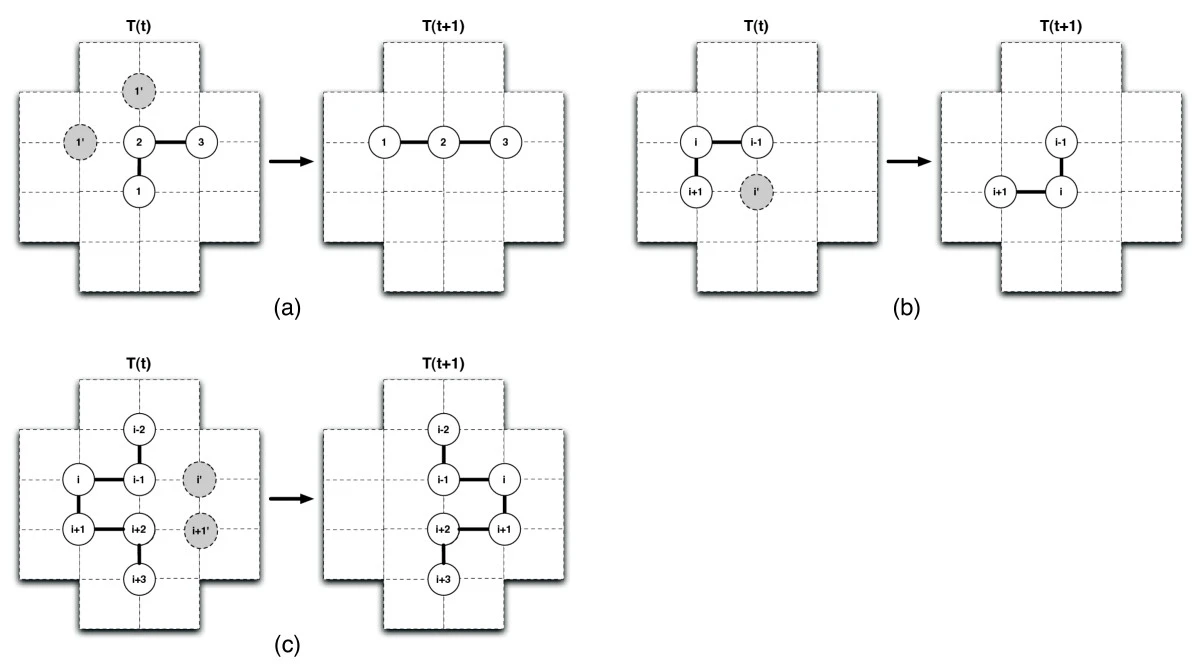
\includegraphics[width=.8\textwidth]{figures/VSHD.png}
    \caption{Mouvements VSHD. En 1a, deux positions sont possibles pour le résidu 1, indiquées par les cercles gris. Si une position ou plusieurs positions s'avèrent être libres, le résidu est déplacé au hasard. En 1b, il n'y a qu'une seule nouvelle position potentielle pour un déplacement de type corner. La position doit se trouver sur le plan formé par i - 1, i et i + 1. Enfin, 1c montre le cas d'un mouvement de crankshaft. Ici deux résidus font une rotation autour d'un axe.}
    \label{fig:VSHD}
\end{figure}

\begin{figure}[H]
    \centering
    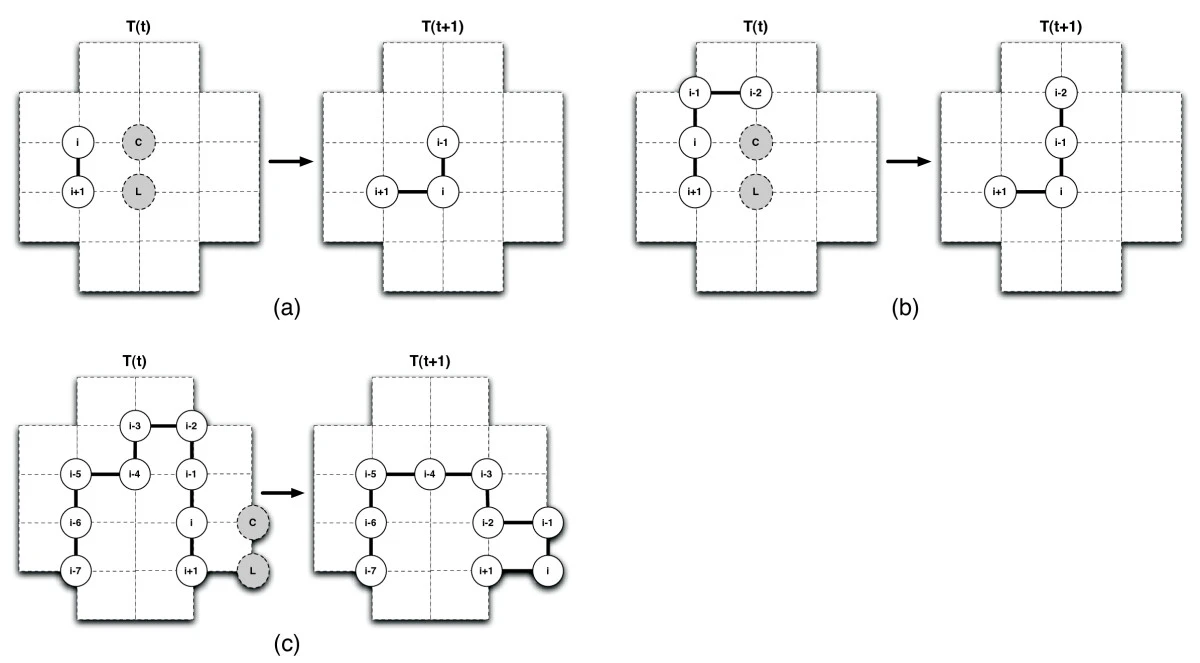
\includegraphics[width=.8\textwidth]{figures/pull.png}
    \caption{Mouvements pull. En 2a, le cas le plus simple où la position C est occupée par le résidu i - 1 est montré. Ce mouvement est équivalent à un mouvement de coin dans le jeu de mouvements VSHD. En 2b, le résidu i est déplacé vers L et i - 1 vers C. La chaîne est dans une conformation valide et le déplacement est terminé. En 2c, les résidus i jusqu'à i - 3 doivent être tirés jusqu'à ce qu'une conformation valide soit trouvée.}
    \label{fig:pull}
\end{figure}

Chaque mouvement peut apporter des modifications à l'énergie totale de la grille, ces modifications vont déterminer sont acceptation. La probabilité d'appliquer un changement est alors définie par la probabilité suivante:

\begin{center}
    $Pr[c\rightarrow {c}'] := \left\{\begin{matrix}
    1 & si \; \Delta E\leq 0,\\
    e^{\frac{-\Delta E}{T\cdot K_b}} & sinon.
    \end{matrix}\right.$    
\end{center}

où $\Delta E := E({c}') - E(c)$ est la différence d'énergie entres les conformations ${c}'$ et $c$, $T$ est la température et $K_b$ est la constante de Boltzmann.

Ainsi, dans un cas peu défavorable, la différence d'énergie sera proche de 0 mais positive. L'exponentielle sera alors plus proche de 1 et il y a alors des chances d'accepter néanmoins le mouvement. A l'inverse, avec une différence d'énergie très positive (très en défaveur de la nouvelle conformation) alors l’exponentielle serait plus proche de 0 et le changement moins probable. C'est ce mécanisme qui permet  à l'algorithme de Monte Carlo de sortir de minima locaux.

Nous implémenterons aussi un algorithme de Monte Carlo avec échange de réplicas. Ici nous lancerons $\chi$ simulations à travers $\chi$ réplicas. Chaque réplica a une température qui lui est associé, déterminant alors sa liberté de mouvement. Il est possible d'échanger deux réplica et ainsi d'échanger leur températures :

\begin{center}
\begin{align*}
    Pr[c\rightarrow {c}'] &:= Pr[l(c_i)\leftrightarrow l(c_j)]\\
    &:= \left\{\begin{matrix}
    1 & si \; \Delta \leq 0,\\
    e^{-\Delta} & otherwise.
    \end{matrix}\right.
\end{align*}
\end{center}

où $\Delta$ est le produit de la différence d'énergie et de la différence de température inverse :

\begin{center}
    $\Delta := (\beta_j-\beta_i)\times (E(c_i)-E(c_j))$
\end{center}

où $\beta_i = \frac{1}{T_i \cdot K_b}$ est l'inverse de la température du réplica.

L'implémentation de cet algorithme a été réalisée en python (3.10). Cela a permis une implémentation orientée objet à travers quatre classes principales, \texttt{Residue}, \texttt{Protein}, \texttt{Lattice} et \texttt{Movement}. Les deux algorithmes que sont celui de Monte Carlo et celui du Replica Exchange Monte Carlo ont été implémenté à travers deux fonctions. La compléxité et lenteur de ce programme vient en grande partie de la représentation des conformation, passant par des matrices, devant être copiées récursivement à chaque calcul de mouvement.

\section{Résultats}

La performance du programme limitant le nombre d'itération qu'il est possible de réaliser le repliements sont loin de ceux attendus et les énergies obtenues sont au maximum moitié moindre que celles attendues.

\begin{table}[H]
    \centering
    \begin{tabular}{c|c|c|c}
        ID & $E^*$ & MC & REMC \\
        S1 & -9 & -4 & -4\\
        S2 & -9 & -4 & -3\\
        S3 & -8 & -3 & -1\\
        S4 & -14 & -3 & -1
    \end{tabular}
    \caption{Résultat des simulations sur les protéines de benchmark}
    \label{tab:my_label}
\end{table}

Toutes les simulations ci-dessus ont été obtenues avec les paramètres suivants :
\begin{itemize}
    \item MC : n-steps=5000, temperature=200
    \item REMC : n-replica=5, max-steps=500, local-steps=100, temperature-min=160, temperature-max=220
\end{itemize}

Les limites de cet algorithme sont notamment dues à la position initiale ne laissant que peu de liberté de mouvement. Nous pouvons suspecter des erreur dans l'implémentation des mouvements pull, qui permettrait pourtant une bien meilleur mobilité. 

\section{Discussion}

La réalisation de ce projet a soulevé plusieurs difficultés. Premièrement les simulations deviennent extrêmement lentes à mesure que le nombre d'itération augmente. Python ne semble alors pas adapté pour ce genre d'implémentation à l'instar de langages compilés tels que le C++, utilisé par les auteurs de l'article.

Le peu de temps dont nous disposions ne nous a pas permis de développer de bonnes pratiques de programmation. Notamment l'implémentation systématiques de tests (à travers pytest), permettant la création d'exemples reproductibles. Mais aussi le calcul du temps de calcul par simulation ou bien mettre en place des simulation non aléatoires.

Enfin une autre difficulté fût la correction d'erreurs de l'article. En effet il ne fait pas mention de l'utilisation de la constante de Boltzmann. Cette constante est cependant utilisée dans le programme lié à l'article, même si la valeur utilisée correspond à la dimension en $kcal/molK$, dimension étrange à l'instar de la dimension classique de cette constante qu'est le $J/K$.

\label{sec:end}

\newpage
\pagestyle{empty}

\begin{appendices}
    \appendixheaderon
    \singlespacing

    \section{Structure du code}
    \begin{figure}[H]
        \centering
        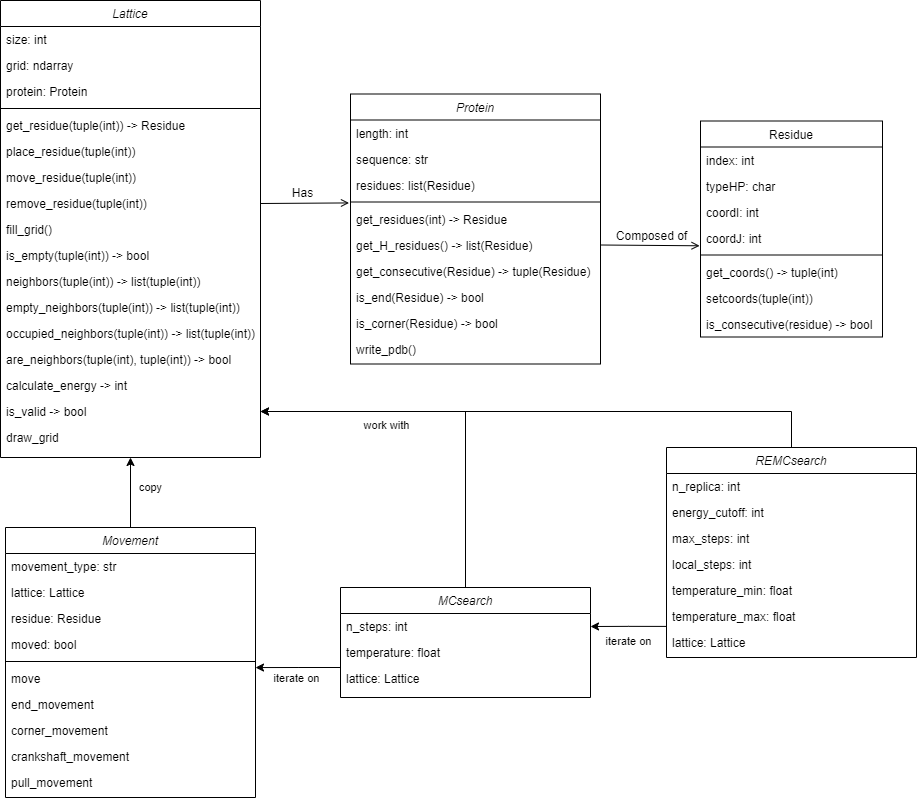
\includegraphics[width=\textwidth]{figures/class_dependencies.png}
        \caption{Structure des classes et fonctions principales}
        \label{fig:class_dependencies}
    \end{figure}

    \section{Sorties des runs de benchmarking}
    \begin{verbatim}
Running test case: HPHPPHHPHPPHPHHPPHPH with optimal energy: -9
Running MC with parameters: n-steps=5000, temperature=200
Final lattice with energy of -4
+-----------+
|           |
|        PP |
| PH     HH |
| HHHPHHPHP |
| PP  PP  H |
|           |
+-----------+
Running REMC with parameters: n-replica=5, energy-cutoff=-9, max-steps=1000, local-steps=100, temperature-min=160, temperature-max=220
Final lattice with energy of -4
+--------------+
|              |
| PH        PP |
| HHHPHPPHPHHH |
| PP        HP |
|              |
+--------------+
\end{verbatim}

\begin{verbatim}
Running test case: HHPPHPPHPPHPPHPPHPPHPPHH with optimal energy: -9
Running MC with parameters: n-steps=5000, temperature=200
Final lattice with energy of -4
+------------------+
|                  |
|             PPHP |
| HHPPHPPHHPPHHHHP |
|        PP  PP    |
|                  |
+------------------+
Running REMC with parameters: n-replica=5, energy-cutoff=-9, max-steps=500, local-steps=100, temperature-min=160, temperature-max=220
Final lattice with energy of -3
+-------------------+
|                   |
| HPP           PP  |
| HHHPPHPPHPPHPPHHH |
| PP                |
|                   |
+-------------------+
\end{verbatim}

\begin{verbatim}
Running test case: PPHPPHHPPPPHHPPPPHHPPPPHH with optimal energy: -8
Running MC with parameters: n-steps=5000, temperature=200
Final lattice with energy of -3
+---------+
|         |
|  PP     |
| PPP PH  |
| PHH PHP |
| HHHPPPP |
| PP   P  |
|     HH  |
|         |
+---------+
Running REMC with parameters: n-replica=5, energy-cutoff=-8, max-steps=500, local-steps=100, temperature-min=160, temperature-max=220
Final lattice with energy of -1
+----------------------+
|                      |
| PP               PHH |
| HHHPPPPHHPPPPHHPPP   |
| P                    |
| P                    |
|                      |
+----------------------+
\end{verbatim}

\end{appendices}

\textit{The source code for this paper is openly available in a github repository, you can access it \href{https://github.com/nobabar/Monte-Carlo-HP-Protein-Folding}{here}.}

\textit{This document was written in \LaTeX  and generated by \href{https://fr.overleaf.com/for/authors}{overleaf}, you can find the source code \href{https://www.overleaf.com/read/mqbxpcbpgqsk}{here}.}

\end{document}
